Using the entire set of Fourier coefficients computed for comparison sake may not be entirely necessary, 
as a matter of fact it is possible to use a subset of just a few of the coefficients to provide roughly 
the same amount of differentiation capability. Figure \ref{fig:coeffvar} displays the variances of each 
generated set of Fourier Coefficients for the 1,397 viromes included in the study.  

\begin{figure}[h!] 
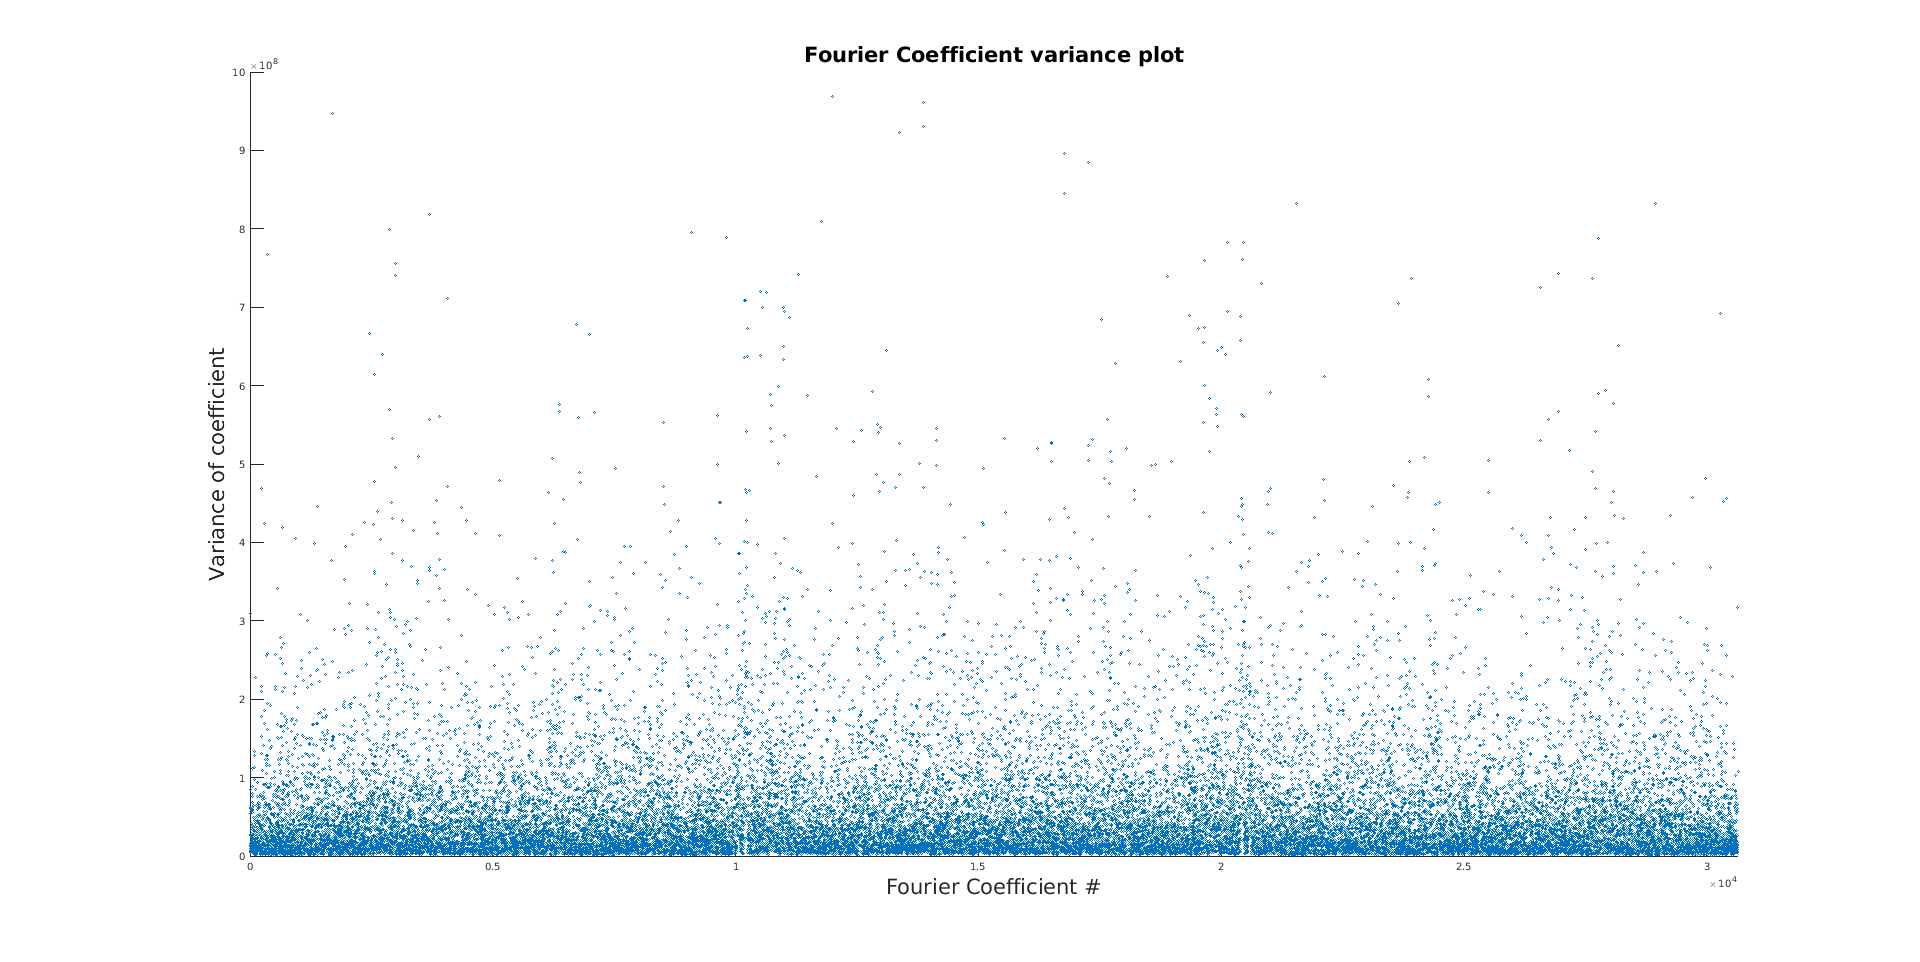
\includegraphics[width=0.5\textwidth]{Images/Files/FCoeff_var.png} 
\caption{A Plot of the Variance of each component among Viromes\label{fig:coeffvar}} 
\end{figure} 

Figure \ref{fig:coeffvar} was produced by first taking the Voss encoded Fourier coefficients that are 
computed for each of the 1,397 total viromes, scaling them each out to the maximal length, such that all 
sets of the Fourier Coefficients were of the same length, and computing the variance for each set of 
coefficients depending on their order of occurrence. On this plot, a filter applied to the coefficients may 
be selected by examining only the coefficients that have a larger variance than some threshold value. 
A histogram of some of the selected coefficients is displayed in Figure \ref{fig:coeffvarhist}. 

\begin{figure}[h!]
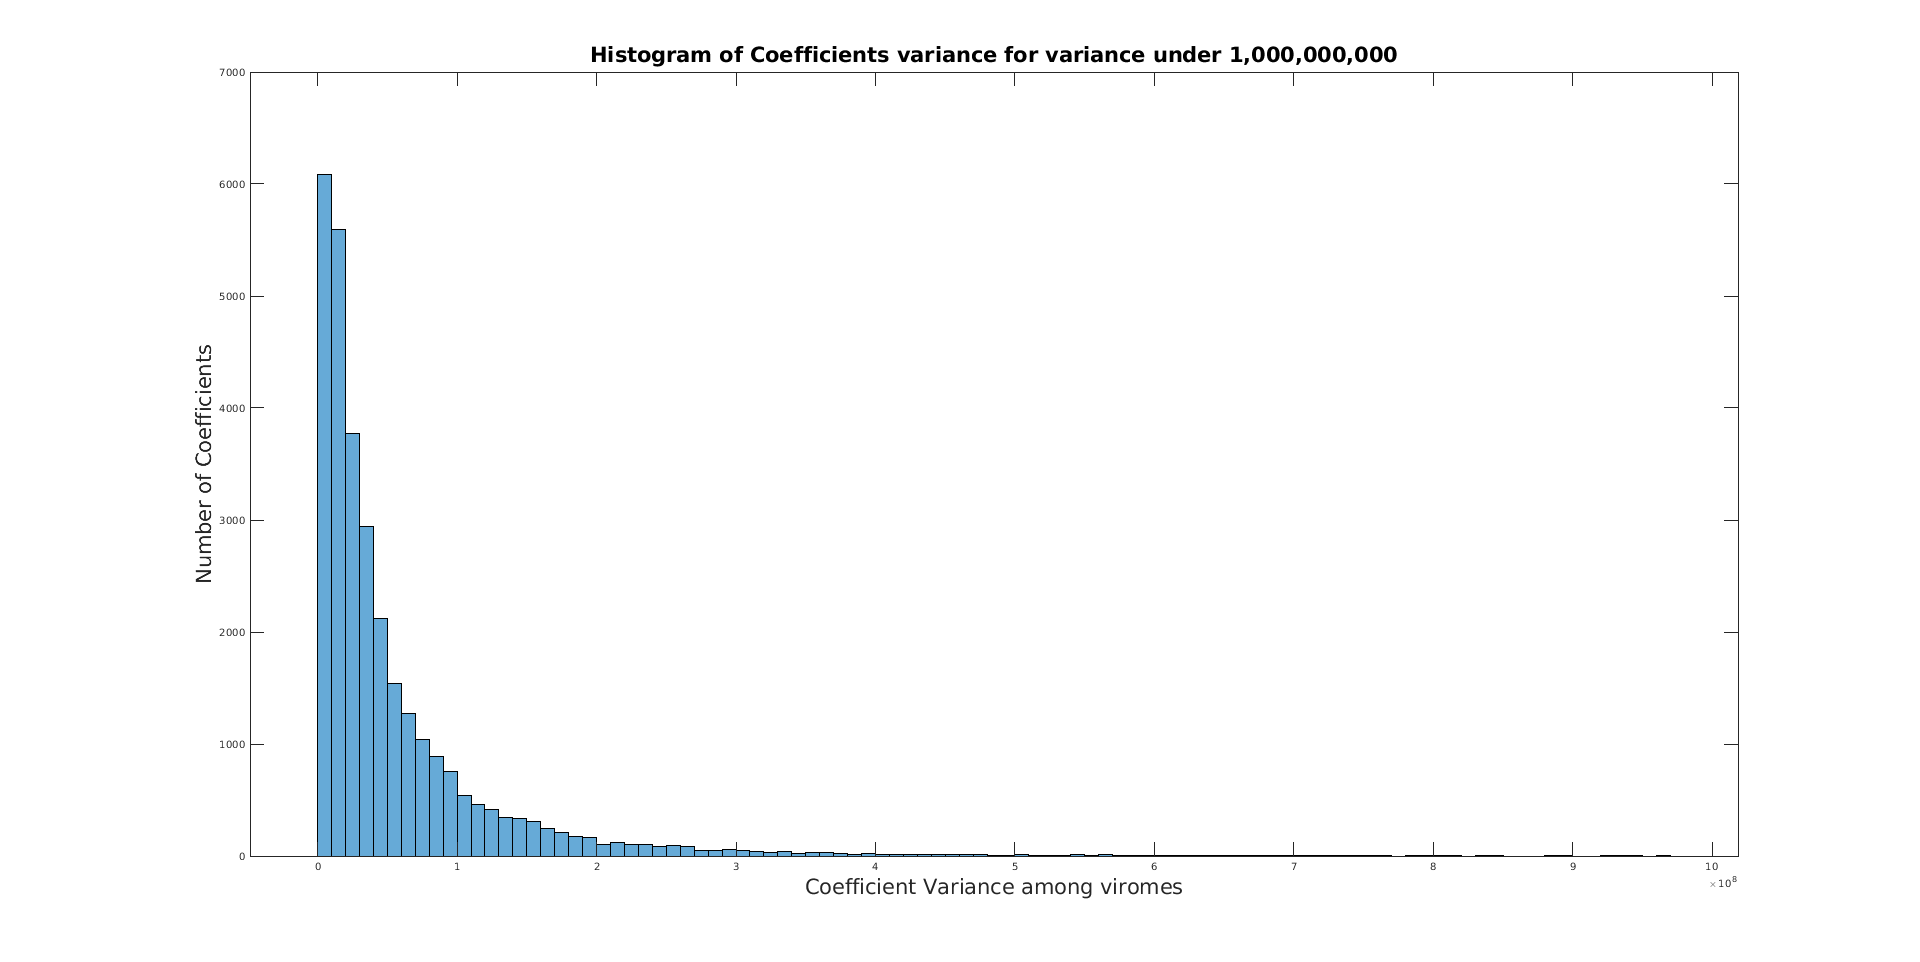
\includegraphics[width=0.5\textwidth]{Images/Files/FCoeff_var_hist.png}
\caption{Histogram of Coefficients by Variance\label{fig:coeffvarhist}}
\end{figure} 

In Figure \ref{fig:coeffvarhist} a filter may be considered as a vertical line at a given variance, beyond which the area
highlighted is the amount of coefficients that are included in the distance calculation phase.  Figure 
\ref{fig:coeffvarsurv} displays the survival curve of coefficients by their variance, that is, the
percentage of coefficients with variance greater than or equal to the ordinate is displayed as the 
abscissa. 

\begin{figure}[h!] 
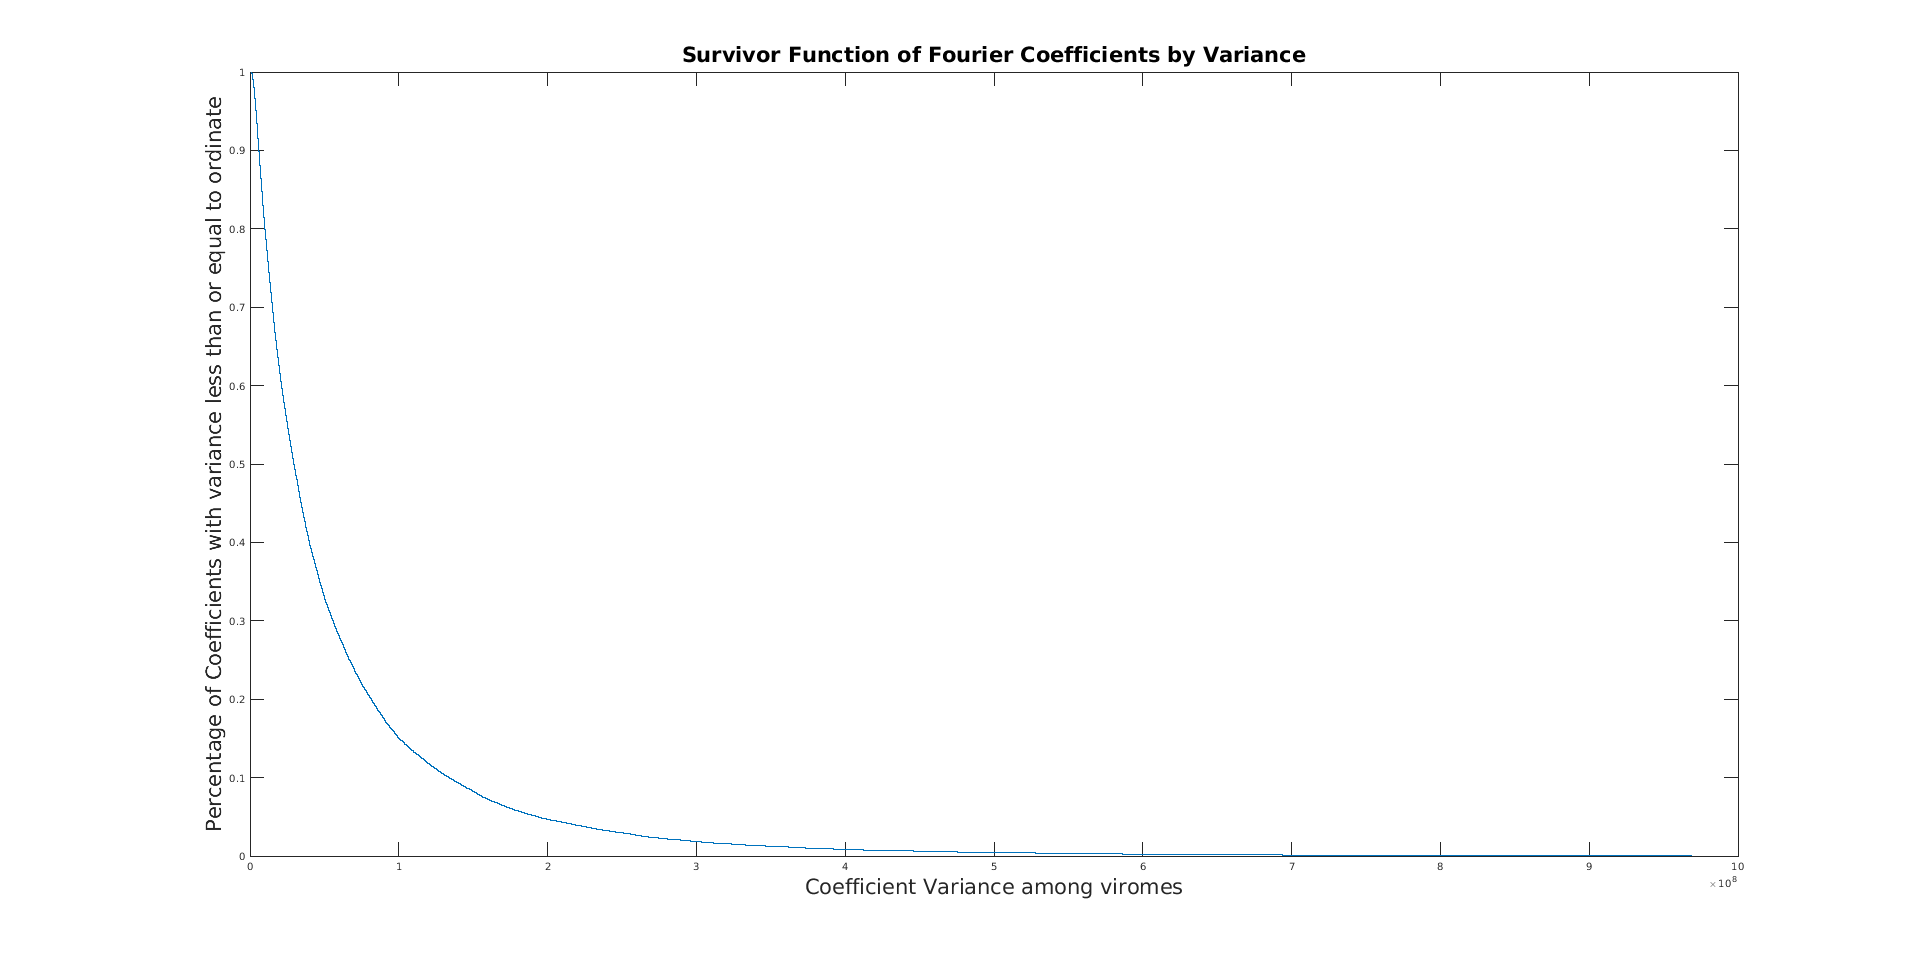
\includegraphics[width=0.5\textwidth]{Images/Files/FCoeff_var_surv.png}
\caption{Survival of Coefficients by Variance\label{fig:coeffvarsurv}}
\end{figure} 

Figure \ref{fig:coeffcorrfilt} displays the correlation of distances computed using pearson's correlation coefficient. 
The correlation is of distances computed using a subset of the coefficients of higher variance than the others, and 
displayed by the percentage of coefficients that are filtered out by variance. 

\begin{figure}[h!] 
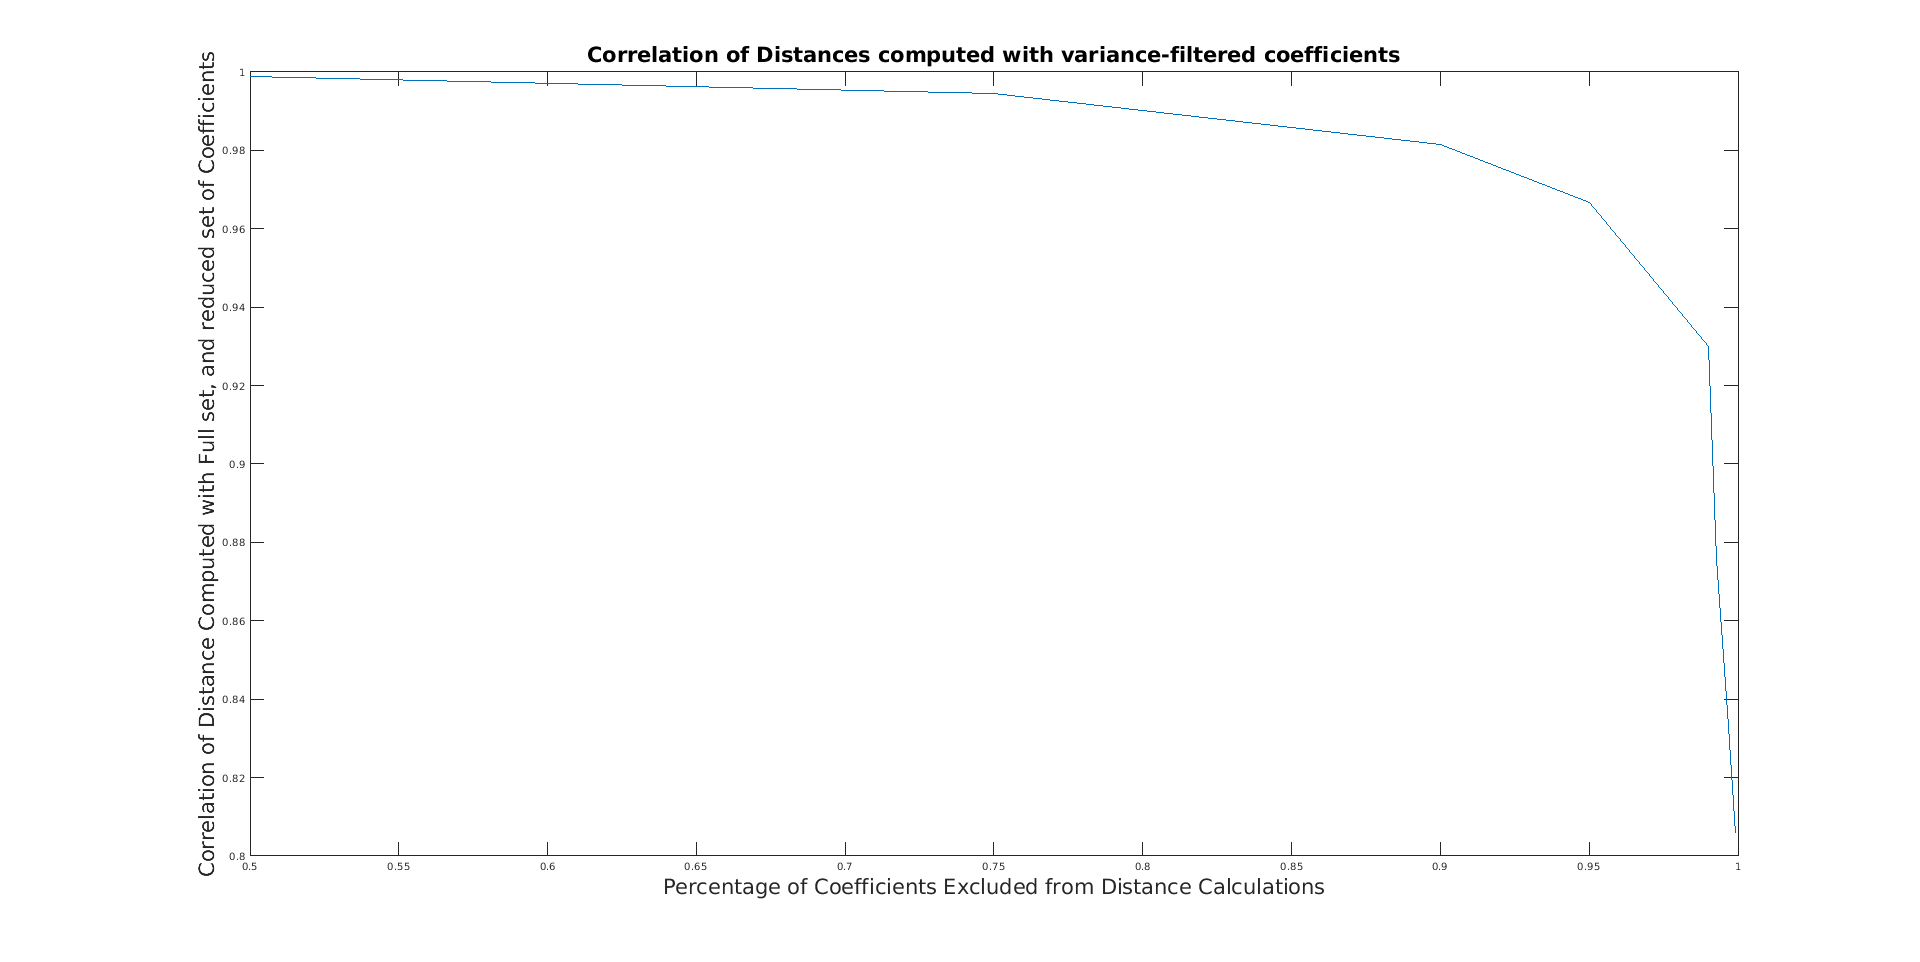
\includegraphics[width=0.5\textwidth]{Images/Files/FCoeff_Correlation_For_Filtered.png}
\caption{ Fourier Coeffients Distance Correlation to distanced computed with all coefficients\label{fig:coeffcorrfilt}} 
\end{figure} 

This filtering process may be considered as semi-analagous to that of a \textit{matched filter} from 
traditional signals processing in the following way.  As a matched filter seeks to exploit a template 
known or suspected, so too does the maximal variance filtering technique discussed here, in that once 
a threshold determination is made then each of the coefficient sequences (for the 1,394 viromes) are
matched to the template determined from the composite variances of the coefficients by selecting only 
those coefficients for which the overall variance was beyond a given threshold to complete the 
Euclidean distances calculation portion of the procedure.  The variance filtering technique does not 
however inspect the composite variances at various lagged values within the sequences, and this is 
where the analogy breaks down.  However, the procedure could accurately be considered akin to the 
\textit{matched filtering} procedure, where only the composite variance at lag zero is used. 

The plot in Figure \ref{fig:coeffcorrfilt} displays the trade-off between filtering more coefficients 
and reflection of distances as they would be computed using the full set of coefficients.  The overall 
distances computed using the coefficients are heavily influenced by the maximum variance coefficient. 
The effect is pronounced to the point that including only this coefficient in the distance calculation 
accounts for 83\% of the variation among distances observed when including all coefficients. 

This investigation reveals that only a single coefficient contains nearly as great an amount of 
information about the overall sequence as the entire set of coefficients, which would allow for 
much faster processing speeds in experiments where a large number of organisms with long sequences are 
involved.  Which leads to the next section, where a consideration of a statistical hypothesis test 
that extends from the distribution analytically described by McGee et al. in \cite{mcg98} is extended 
to test the similarity of genomic sequences. 